\documentclass[1p]{elsarticle_modified}
%\bibliographystyle{elsarticle-num}

%\usepackage[colorlinks]{hyperref}
%\usepackage{abbrmath_seonhwa} %\Abb, \Ascr, \Acal ,\Abf, \Afrak
\usepackage{amsfonts}
\usepackage{amssymb}
\usepackage{amsmath}
\usepackage{amsthm}
\usepackage{scalefnt}
\usepackage{amsbsy}
\usepackage{kotex}
\usepackage{caption}
\usepackage{subfig}
\usepackage{color}
\usepackage{graphicx}
\usepackage{xcolor} %% white, black, red, green, blue, cyan, magenta, yellow
\usepackage{float}
\usepackage{setspace}
\usepackage{hyperref}

\usepackage{tikz}
\usetikzlibrary{arrows}

\usepackage{multirow}
\usepackage{array} % fixed length table
\usepackage{hhline}

%%%%%%%%%%%%%%%%%%%%%
\makeatletter
\renewcommand*\env@matrix[1][\arraystretch]{%
	\edef\arraystretch{#1}%
	\hskip -\arraycolsep
	\let\@ifnextchar\new@ifnextchar
	\array{*\c@MaxMatrixCols c}}
\makeatother %https://tex.stackexchange.com/questions/14071/how-can-i-increase-the-line-spacing-in-a-matrix
%%%%%%%%%%%%%%%

\usepackage[normalem]{ulem}

\newcommand{\msout}[1]{\ifmmode\text{\sout{\ensuremath{#1}}}\else\sout{#1}\fi}
%SOURCE: \msout is \stkout macro in https://tex.stackexchange.com/questions/20609/strikeout-in-math-mode

\newcommand{\cancel}[1]{
	\ifmmode
	{\color{red}\msout{#1}}
	\else
	{\color{red}\sout{#1}}
	\fi
}

\newcommand{\add}[1]{
	{\color{blue}\uwave{#1}}
}

\newcommand{\replace}[2]{
	\ifmmode
	{\color{red}\msout{#1}}{\color{blue}\uwave{#2}}
	\else
	{\color{red}\sout{#1}}{\color{blue}\uwave{#2}}
	\fi
}

\newcommand{\Sol}{\mathcal{S}} %segment
\newcommand{\D}{D} %diagram
\newcommand{\A}{\mathcal{A}} %arc


%%%%%%%%%%%%%%%%%%%%%%%%%%%%%5 test

\def\sl{\operatorname{\textup{SL}}(2,\Cbb)}
\def\psl{\operatorname{\textup{PSL}}(2,\Cbb)}
\def\quan{\mkern 1mu \triangleright \mkern 1mu}

\theoremstyle{definition}
\newtheorem{thm}{Theorem}[section]
\newtheorem{prop}[thm]{Proposition}
\newtheorem{lem}[thm]{Lemma}
\newtheorem{ques}[thm]{Question}
\newtheorem{cor}[thm]{Corollary}
\newtheorem{defn}[thm]{Definition}
\newtheorem{exam}[thm]{Example}
\newtheorem{rmk}[thm]{Remark}
\newtheorem{alg}[thm]{Algorithm}

\newcommand{\I}{\sqrt{-1}}
\begin{document}

%\begin{frontmatter}
%
%\title{Boundary parabolic representations of knots up to 8 crossings}
%
%%% Group authors per affiliation:
%\author{Yunhi Cho} 
%\address{Department of Mathematics, University of Seoul, Seoul, Korea}
%\ead{yhcho@uos.ac.kr}
%
%
%\author{Seonhwa Kim} %\fnref{s_kim}}
%\address{Center for Geometry and Physics, Institute for Basic Science, Pohang, 37673, Korea}
%\ead{ryeona17@ibs.re.kr}
%
%\author{Hyuk Kim}
%\address{Department of Mathematical Sciences, Seoul National University, Seoul 08826, Korea}
%\ead{hyukkim@snu.ac.kr}
%
%\author{Seokbeom Yoon}
%\address{Department of Mathematical Sciences, Seoul National University, Seoul, 08826,  Korea}
%\ead{sbyoon15@snu.ac.kr}
%
%\begin{abstract}
%We find all boundary parabolic representation of knots up to 8 crossings.
%
%\end{abstract}
%\begin{keyword}
%    \MSC[2010] 57M25 
%\end{keyword}
%
%\end{frontmatter}

%\linenumbers
%\tableofcontents
%
\newcommand\colored[1]{\textcolor{white}{\rule[-0.35ex]{0.8em}{1.4ex}}\kern-0.8em\color{red} #1}%
%\newcommand\colored[1]{\textcolor{white}{ #1}\kern-2.17ex	\textcolor{white}{ #1}\kern-1.81ex	\textcolor{white}{ #1}\kern-2.15ex\color{red}#1	}

{\Large $\underline{11a_{123}~(K11a_{123})}$}

\setlength{\tabcolsep}{10pt}
\renewcommand{\arraystretch}{1.6}
\vspace{1cm}\begin{tabular}{m{100pt}>{\centering\arraybackslash}m{274pt}}
\multirow{5}{120pt}{
	\centering
	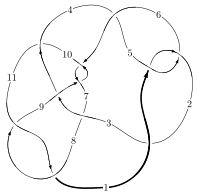
\includegraphics[width=112pt]{../../../GIT/diagram.site/Diagrams/png/372_11a_123.png}\\
\ \ \ A knot diagram\footnotemark}&
\allowdisplaybreaks
\textbf{Linearized knot diagam} \\
\cline{2-2}
 &
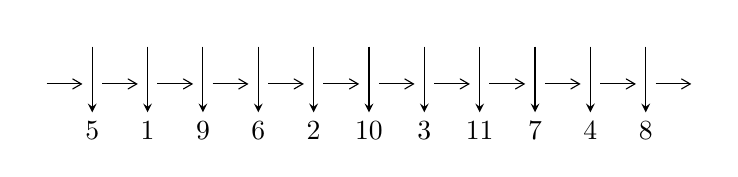
\begin{tikzpicture}[x=20pt, y=17pt]
	% nodes
	\node (C0) at (0, 0) {};
	\node (C1) at (1, 0) {};
	\node (C1U) at (1, +1) {};
	\node (C1D) at (1, -1) {5};

	\node (C2) at (2, 0) {};
	\node (C2U) at (2, +1) {};
	\node (C2D) at (2, -1) {1};

	\node (C3) at (3, 0) {};
	\node (C3U) at (3, +1) {};
	\node (C3D) at (3, -1) {9};

	\node (C4) at (4, 0) {};
	\node (C4U) at (4, +1) {};
	\node (C4D) at (4, -1) {6};

	\node (C5) at (5, 0) {};
	\node (C5U) at (5, +1) {};
	\node (C5D) at (5, -1) {2};

	\node (C6) at (6, 0) {};
	\node (C6U) at (6, +1) {};
	\node (C6D) at (6, -1) {10};

	\node (C7) at (7, 0) {};
	\node (C7U) at (7, +1) {};
	\node (C7D) at (7, -1) {3};

	\node (C8) at (8, 0) {};
	\node (C8U) at (8, +1) {};
	\node (C8D) at (8, -1) {11};

	\node (C9) at (9, 0) {};
	\node (C9U) at (9, +1) {};
	\node (C9D) at (9, -1) {7};

	\node (C10) at (10, 0) {};
	\node (C10U) at (10, +1) {};
	\node (C10D) at (10, -1) {4};

	\node (C11) at (11, 0) {};
	\node (C11U) at (11, +1) {};
	\node (C11D) at (11, -1) {8};
	\node (C12) at (12, 0) {};

	% arrows
	\draw[->,>={angle 60}]
	(C0) edge (C1) (C1) edge (C2) (C2) edge (C3) (C3) edge (C4) (C4) edge (C5) (C5) edge (C6) (C6) edge (C7) (C7) edge (C8) (C8) edge (C9) (C9) edge (C10) (C10) edge (C11) (C11) edge (C12) ;	\draw[->,>=stealth]
	(C1U) edge (C1D) (C2U) edge (C2D) (C3U) edge (C3D) (C4U) edge (C4D) (C5U) edge (C5D) (C6U) edge (C6D) (C7U) edge (C7D) (C8U) edge (C8D) (C9U) edge (C9D) (C10U) edge (C10D) (C11U) edge (C11D) ;
	\end{tikzpicture} \\
\hhline{~~} \\& 
\textbf{Solving Sequence} \\ \cline{2-2} 
 &
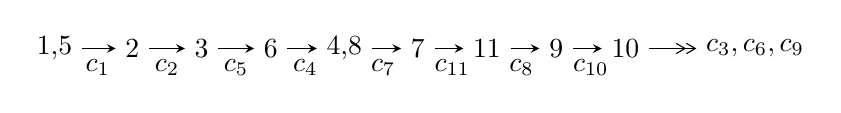
\begin{tikzpicture}[x=25pt, y=7pt]
	% node
	\node (A0) at (-1/8, 0) {1,5};
	\node (A1) at (1, 0) {2};
	\node (A2) at (2, 0) {3};
	\node (A3) at (3, 0) {6};
	\node (A4) at (65/16, 0) {4,8};
	\node (A5) at (41/8, 0) {7};
	\node (A6) at (49/8, 0) {11};
	\node (A7) at (57/8, 0) {9};
	\node (A8) at (65/8, 0) {10};
	\node (C1) at (1/2, -1) {$c_{1}$};
	\node (C2) at (3/2, -1) {$c_{2}$};
	\node (C3) at (5/2, -1) {$c_{5}$};
	\node (C4) at (7/2, -1) {$c_{4}$};
	\node (C5) at (37/8, -1) {$c_{7}$};
	\node (C6) at (45/8, -1) {$c_{11}$};
	\node (C7) at (53/8, -1) {$c_{8}$};
	\node (C8) at (61/8, -1) {$c_{10}$};
	\node (A9) at (10, 0) {$c_{3},c_{6},c_{9}$};

	% edge
	\draw[->,>=stealth]	
	(A0) edge (A1) (A1) edge (A2) (A2) edge (A3) (A3) edge (A4) (A4) edge (A5) (A5) edge (A6) (A6) edge (A7) (A7) edge (A8) ;
	\draw[->>,>={angle 60}]	
	(A8) edge (A9);
\end{tikzpicture} \\ 

\end{tabular} \\

\footnotetext{
The image of knot diagram is generated by the software ``\textbf{Draw programme}" developed by Andrew Bartholomew(\url{http://www.layer8.co.uk/maths/draw/index.htm\#Running-draw}), where we modified some parts for our purpose(\url{https://github.com/CATsTAILs/LinksPainter}).
}\phantom \\ \newline 
\centering \textbf{Ideals for irreducible components\footnotemark of $X_{\text{par}}$} 
 
\begin{align*}
I^u_{1}&=\langle 
31496267249 u^{24}-1954119851 u^{23}+\cdots+353576605306 b-294716823050,\\
\phantom{I^u_{1}}&\phantom{= \langle  }-258242463245 u^{24}+140426199118 u^{23}+\cdots+707153210612 a+177949498093,\\
\phantom{I^u_{1}}&\phantom{= \langle  }u^{25}-2 u^{24}+\cdots+17 u-4\rangle \\
I^u_{2}&=\langle 
-5 u^{18} a-45 u^{18}+\cdots+27 a+5,\;-6 u^{18} a+26 u^{18}+\cdots-6 a+39,\;u^{19}- u^{18}+\cdots+u^2-1\rangle \\
I^u_{3}&=\langle 
b+1,\;2 a+2 u+1,\;u^3+u^2-1\rangle \\
I^u_{4}&=\langle 
b- a-1,\;a^2+2 a+2,\;u-1\rangle \\
\\
\end{align*}
\raggedright * 4 irreducible components of $\dim_{\mathbb{C}}=0$, with total 68 representations.\\
\footnotetext{All coefficients of polynomials are rational numbers. But the coefficients are sometimes approximated in decimal forms when there is not enough margin.}
\newpage
\renewcommand{\arraystretch}{1}
\centering \section*{I. $I^u_{1}= \langle 3.15\times10^{10} u^{24}-1.95\times10^{9} u^{23}+\cdots+3.54\times10^{11} b-2.95\times10^{11},\;-2.58\times10^{11} u^{24}+1.40\times10^{11} u^{23}+\cdots+7.07\times10^{11} a+1.78\times10^{11},\;u^{25}-2 u^{24}+\cdots+17 u-4 \rangle$}
\flushleft \textbf{(i) Arc colorings}\\
\begin{tabular}{m{7pt} m{180pt} m{7pt} m{180pt} }
\flushright $a_{1}=$&$\begin{pmatrix}1\\0\end{pmatrix}$ \\
\flushright $a_{5}=$&$\begin{pmatrix}0\\u\end{pmatrix}$ \\
\flushright $a_{2}=$&$\begin{pmatrix}1\\u^2\end{pmatrix}$ \\
\flushright $a_{3}=$&$\begin{pmatrix}- u^2+1\\u^2\end{pmatrix}$ \\
\flushright $a_{6}=$&$\begin{pmatrix}- u\\- u^3+u\end{pmatrix}$ \\
\flushright $a_{4}=$&$\begin{pmatrix}u^3\\u^5- u^3+u\end{pmatrix}$ \\
\flushright $a_{8}=$&$\begin{pmatrix}0.365186 u^{24}-0.198580 u^{23}+\cdots-5.28891 u-0.251642\\-0.0890790 u^{24}+0.00552672 u^{23}+\cdots-1.23519 u+0.833530\end{pmatrix}$ \\
\flushright $a_{7}=$&$\begin{pmatrix}0.267603 u^{24}-0.170382 u^{23}+\cdots-4.06703 u-0.0336839\\-0.227826 u^{24}+0.244721 u^{23}+\cdots+1.30904 u+0.0124582\end{pmatrix}$ \\
\flushright $a_{11}=$&$\begin{pmatrix}-0.361710 u^{24}+0.276963 u^{23}+\cdots+5.53501 u+0.291576\\0.135603 u^{24}-0.0416754 u^{23}+\cdots+1.55999 u-0.715415\end{pmatrix}$ \\
\flushright $a_{9}=$&$\begin{pmatrix}0.690139 u^{24}-0.455342 u^{23}+\cdots-9.24059 u-0.0115544\\-0.314729 u^{24}+0.224657 u^{23}+\cdots-1.21944 u+0.939187\end{pmatrix}$ \\
\flushright $a_{10}=$&$\begin{pmatrix}-0.323410 u^{24}+0.155971 u^{23}+\cdots+3.99738 u+0.846565\\0.110684 u^{24}-0.103445 u^{23}+\cdots+0.590987 u-0.502652\end{pmatrix}$\\ \flushright $a_{10}=$&$\begin{pmatrix}-0.323410 u^{24}+0.155971 u^{23}+\cdots+3.99738 u+0.846565\\0.110684 u^{24}-0.103445 u^{23}+\cdots+0.590987 u-0.502652\end{pmatrix}$\\&\end{tabular}
\flushleft \textbf{(ii) Obstruction class $= -1$}\\~\\
\flushleft \textbf{(iii) Cusp Shapes $= -\frac{781324937945}{707153210612} u^{24}-\frac{104635078433}{707153210612} u^{23}+\cdots+\frac{4120329941333}{176788302653} u-\frac{3444311623734}{176788302653}$}\\~\\
\newpage\renewcommand{\arraystretch}{1}
\flushleft \textbf{(iv) u-Polynomials at the component}\newline \\
\begin{tabular}{m{50pt}|m{274pt}}
Crossings & \hspace{64pt}u-Polynomials at each crossing \\
\hline $$\begin{aligned}c_{1},c_{5}\end{aligned}$$&$\begin{aligned}
&u^{25}+2 u^{24}+\cdots+17 u+4
\end{aligned}$\\
\hline $$\begin{aligned}c_{2},c_{4}\end{aligned}$$&$\begin{aligned}
&u^{25}+8 u^{24}+\cdots+241 u+16
\end{aligned}$\\
\hline $$\begin{aligned}c_{3}\end{aligned}$$&$\begin{aligned}
&u^{25}-3 u^{24}+\cdots-96 u+128
\end{aligned}$\\
\hline $$\begin{aligned}c_{6},c_{8},c_{9}\\c_{11}\end{aligned}$$&$\begin{aligned}
&u^{25}+3 u^{24}+\cdots+2 u+1
\end{aligned}$\\
\hline $$\begin{aligned}c_{7},c_{10}\end{aligned}$$&$\begin{aligned}
&8(8 u^{25}+4 u^{24}+\cdots+2 u+2)
\end{aligned}$\\
\hline
\end{tabular}\\~\\
\newpage\renewcommand{\arraystretch}{1}
\flushleft \textbf{(v) Riley Polynomials at the component}\newline \\
\begin{tabular}{m{50pt}|m{274pt}}
Crossings & \hspace{64pt}Riley Polynomials at each crossing \\
\hline $$\begin{aligned}c_{1},c_{5}\end{aligned}$$&$\begin{aligned}
&y^{25}-8 y^{24}+\cdots+241 y-16
\end{aligned}$\\
\hline $$\begin{aligned}c_{2},c_{4}\end{aligned}$$&$\begin{aligned}
&y^{25}+20 y^{24}+\cdots+19233 y-256
\end{aligned}$\\
\hline $$\begin{aligned}c_{3}\end{aligned}$$&$\begin{aligned}
&y^{25}+9 y^{24}+\cdots-72704 y-16384
\end{aligned}$\\
\hline $$\begin{aligned}c_{6},c_{8},c_{9}\\c_{11}\end{aligned}$$&$\begin{aligned}
&y^{25}+17 y^{24}+\cdots+16 y-1
\end{aligned}$\\
\hline $$\begin{aligned}c_{7},c_{10}\end{aligned}$$&$\begin{aligned}
&64(64 y^{25}+1072 y^{24}+\cdots+20 y-4)
\end{aligned}$\\
\hline
\end{tabular}\\~\\
\newpage\flushleft \textbf{(vi) Complex Volumes and Cusp Shapes}
$$\begin{array}{c|c|c}  
\text{Solutions to }I^u_{1}& \I (\text{vol} + \sqrt{-1}CS) & \text{Cusp shape}\\
 \hline 
\begin{aligned}
u &= \phantom{-}0.831869 + 0.519995 I \\
a &= \phantom{-}0.60247 - 1.53377 I \\
b &= \phantom{-}0.604789 + 0.633838 I\end{aligned}
 & -0.94821 - 3.43572 I & -13.2032 + 6.7534 I \\ \hline\begin{aligned}
u &= \phantom{-}0.831869 - 0.519995 I \\
a &= \phantom{-}0.60247 + 1.53377 I \\
b &= \phantom{-}0.604789 - 0.633838 I\end{aligned}
 & -0.94821 + 3.43572 I & -13.2032 - 6.7534 I \\ \hline\begin{aligned}
u &= -0.096629 + 0.930099 I \\
a &= \phantom{-}0.10164 + 1.51799 I \\
b &= -0.269095 - 1.312200 I\end{aligned}
 & \phantom{-}7.47156 - 5.57189 I & -2.30391 + 4.65826 I \\ \hline\begin{aligned}
u &= -0.096629 - 0.930099 I \\
a &= \phantom{-}0.10164 - 1.51799 I \\
b &= -0.269095 + 1.312200 I\end{aligned}
 & \phantom{-}7.47156 + 5.57189 I & -2.30391 - 4.65826 I \\ \hline\begin{aligned}
u &= -0.873066 + 0.713586 I \\
a &= -0.343451 - 0.174556 I \\
b &= -0.321236 - 0.053568 I\end{aligned}
 & \phantom{-}2.48771 + 2.73173 I & -3.19620 - 2.74281 I \\ \hline\begin{aligned}
u &= -0.873066 - 0.713586 I \\
a &= -0.343451 + 0.174556 I \\
b &= -0.321236 + 0.053568 I\end{aligned}
 & \phantom{-}2.48771 - 2.73173 I & -3.19620 + 2.74281 I \\ \hline\begin{aligned}
u &= \phantom{-}0.890108 + 0.788825 I \\
a &= -0.718513 - 0.942420 I \\
b &= \phantom{-}1.43833 - 0.04819 I\end{aligned}
 & \phantom{-}2.16301 - 2.96631 I & -1.51503 + 3.55668 I \\ \hline\begin{aligned}
u &= \phantom{-}0.890108 - 0.788825 I \\
a &= -0.718513 + 0.942420 I \\
b &= \phantom{-}1.43833 + 0.04819 I\end{aligned}
 & \phantom{-}2.16301 + 2.96631 I & -1.51503 - 3.55668 I \\ \hline\begin{aligned}
u &= \phantom{-}0.746418 + 0.296773 I \\
a &= -0.848177 + 0.452473 I \\
b &= \phantom{-}0.188697 - 0.408041 I\end{aligned}
 & -0.644117 - 0.222126 I & -12.29988 - 0.69416 I \\ \hline\begin{aligned}
u &= \phantom{-}0.746418 - 0.296773 I \\
a &= -0.848177 - 0.452473 I \\
b &= \phantom{-}0.188697 + 0.408041 I\end{aligned}
 & -0.644117 + 0.222126 I & -12.29988 + 0.69416 I\\
 \hline 
 \end{array}$$\newpage$$\begin{array}{c|c|c}  
\text{Solutions to }I^u_{1}& \I (\text{vol} + \sqrt{-1}CS) & \text{Cusp shape}\\
 \hline 
\begin{aligned}
u &= -0.791605 + 0.124227 I \\
a &= \phantom{-}1.178100 + 0.337562 I \\
b &= \phantom{-}1.040980 + 0.275015 I\end{aligned}
 & -2.97368 + 0.31797 I & -15.9411 - 13.1085 I \\ \hline\begin{aligned}
u &= -0.791605 - 0.124227 I \\
a &= \phantom{-}1.178100 - 0.337562 I \\
b &= \phantom{-}1.040980 - 0.275015 I\end{aligned}
 & -2.97368 - 0.31797 I & -15.9411 + 13.1085 I \\ \hline\begin{aligned}
u &= -1.142430 + 0.382078 I \\
a &= -1.268030 - 0.422167 I \\
b &= -0.409233 + 1.264710 I\end{aligned}
 & \phantom{-}3.90197 + 10.08690 I & -8.02551 - 8.45672 I \\ \hline\begin{aligned}
u &= -1.142430 - 0.382078 I \\
a &= -1.268030 + 0.422167 I \\
b &= -0.409233 - 1.264710 I\end{aligned}
 & \phantom{-}3.90197 - 10.08690 I & -8.02551 + 8.45672 I \\ \hline\begin{aligned}
u &= \phantom{-}0.770950 + 0.937113 I \\
a &= \phantom{-}0.30856 - 1.63900 I \\
b &= -0.48655 + 1.44328 I\end{aligned}
 & \phantom{-}12.8491 + 9.5213 I & -4.07416 - 4.01278 I \\ \hline\begin{aligned}
u &= \phantom{-}0.770950 - 0.937113 I \\
a &= \phantom{-}0.30856 + 1.63900 I \\
b &= -0.48655 - 1.44328 I\end{aligned}
 & \phantom{-}12.8491 - 9.5213 I & -4.07416 + 4.01278 I \\ \hline\begin{aligned}
u &= -0.749482 + 1.006980 I \\
a &= -0.24489 - 1.53795 I \\
b &= \phantom{-}0.065690 + 1.341370 I\end{aligned}
 & \phantom{-}11.66030 + 0.32743 I & -0.684836 - 0.302346 I \\ \hline\begin{aligned}
u &= -0.749482 - 1.006980 I \\
a &= -0.24489 + 1.53795 I \\
b &= \phantom{-}0.065690 - 1.341370 I\end{aligned}
 & \phantom{-}11.66030 - 0.32743 I & -0.684836 + 0.302346 I \\ \hline\begin{aligned}
u &= \phantom{-}1.286720 + 0.219140 I \\
a &= \phantom{-}0.295022 - 0.018174 I \\
b &= -0.140637 + 1.182510 I\end{aligned}
 & \phantom{-}2.59539 + 1.53840 I & -3.54408 - 4.89308 I \\ \hline\begin{aligned}
u &= \phantom{-}1.286720 - 0.219140 I \\
a &= \phantom{-}0.295022 + 0.018174 I \\
b &= -0.140637 - 1.182510 I\end{aligned}
 & \phantom{-}2.59539 - 1.53840 I & -3.54408 + 4.89308 I\\
 \hline 
 \end{array}$$\newpage$$\begin{array}{c|c|c}  
\text{Solutions to }I^u_{1}& \I (\text{vol} + \sqrt{-1}CS) & \text{Cusp shape}\\
 \hline 
\begin{aligned}
u &= \phantom{-}1.033460 + 0.815877 I \\
a &= -1.39808 + 1.83834 I \\
b &= -0.53103 - 1.43134 I\end{aligned}
 & \phantom{-}12.0149 - 15.9713 I & -5.35626 + 8.57789 I \\ \hline\begin{aligned}
u &= \phantom{-}1.033460 - 0.815877 I \\
a &= -1.39808 - 1.83834 I \\
b &= -0.53103 + 1.43134 I\end{aligned}
 & \phantom{-}12.0149 + 15.9713 I & -5.35626 - 8.57789 I \\ \hline\begin{aligned}
u &= -1.076920 + 0.848675 I \\
a &= \phantom{-}1.04834 + 1.34169 I \\
b &= \phantom{-}0.153566 - 1.310870 I\end{aligned}
 & \phantom{-}10.62700 + 6.42707 I & -2.25103 - 5.26300 I \\ \hline\begin{aligned}
u &= -1.076920 - 0.848675 I \\
a &= \phantom{-}1.04834 - 1.34169 I \\
b &= \phantom{-}0.153566 + 1.310870 I\end{aligned}
 & \phantom{-}10.62700 - 6.42707 I & -2.25103 + 5.26300 I \\ \hline\begin{aligned}
u &= \phantom{-}0.341201\phantom{ +0.000000I} \\
a &= -1.17598\phantom{ +0.000000I} \\
b &= \phantom{-}0.331472\phantom{ +0.000000I}\end{aligned}
 & -0.684794\phantom{ +0.000000I} & -14.4600\phantom{ +0.000000I}\\
 \hline 
 \end{array}$$\newpage\newpage\renewcommand{\arraystretch}{1}
\centering \section*{II. $I^u_{2}= \langle -5 u^{18} a-45 u^{18}+\cdots+27 a+5,\;-6 u^{18} a+26 u^{18}+\cdots-6 a+39,\;u^{19}- u^{18}+\cdots+u^2-1 \rangle$}
\flushleft \textbf{(i) Arc colorings}\\
\begin{tabular}{m{7pt} m{180pt} m{7pt} m{180pt} }
\flushright $a_{1}=$&$\begin{pmatrix}1\\0\end{pmatrix}$ \\
\flushright $a_{5}=$&$\begin{pmatrix}0\\u\end{pmatrix}$ \\
\flushright $a_{2}=$&$\begin{pmatrix}1\\u^2\end{pmatrix}$ \\
\flushright $a_{3}=$&$\begin{pmatrix}- u^2+1\\u^2\end{pmatrix}$ \\
\flushright $a_{6}=$&$\begin{pmatrix}- u\\- u^3+u\end{pmatrix}$ \\
\flushright $a_{4}=$&$\begin{pmatrix}u^3\\u^5- u^3+u\end{pmatrix}$ \\
\flushright $a_{8}=$&$\begin{pmatrix}a\\0.147059 a u^{18}+1.32353 u^{18}+\cdots-0.794118 a-0.147059\end{pmatrix}$ \\
\flushright $a_{7}=$&$\begin{pmatrix}0.176471 a u^{18}+0.588235 u^{18}+\cdots+0.647059 a-0.176471\\0.205882 a u^{18}+1.85294 u^{18}+\cdots-0.911765 a-0.205882\end{pmatrix}$ \\
\flushright $a_{11}=$&$\begin{pmatrix}1.32353 a u^{18}-4.08824 u^{18}+\cdots-0.147059 a-6.32353\\-0.205882 a u^{18}+0.147059 u^{18}+\cdots-0.0882353 a+0.205882\end{pmatrix}$ \\
\flushright $a_{9}=$&$\begin{pmatrix}u^{18}-3 u^{16}+8 u^{14}-13 u^{12}+17 u^{10}-15 u^8+10 u^6-2 u^4- u^2+1\\- u^{18}+2 u^{16}-5 u^{14}+6 u^{12}-5 u^{10}+2 u^8+2 u^6-4 u^4+u^2\end{pmatrix}$ \\
\flushright $a_{10}=$&$\begin{pmatrix}0.794118 a u^{18}-3.85294 u^{18}+\cdots-0.0882353 a-5.79412\\0.323529 a u^{18}+1.91176 u^{18}+\cdots-0.147059 a+2.67647\end{pmatrix}$\\ \flushright $a_{10}=$&$\begin{pmatrix}0.794118 a u^{18}-3.85294 u^{18}+\cdots-0.0882353 a-5.79412\\0.323529 a u^{18}+1.91176 u^{18}+\cdots-0.147059 a+2.67647\end{pmatrix}$\\&\end{tabular}
\flushleft \textbf{(ii) Obstruction class $= -1$}\\~\\
\flushleft \textbf{(iii) Cusp Shapes $= -4 u^{18}+12 u^{16}-4 u^{15}-32 u^{14}+8 u^{13}+56 u^{12}-20 u^{11}-72 u^{10}+24 u^9+76 u^8-24 u^7-52 u^6+12 u^5+24 u^4-4 u^3-4 u^2-8 u-10$}\\~\\
\newpage\renewcommand{\arraystretch}{1}
\flushleft \textbf{(iv) u-Polynomials at the component}\newline \\
\begin{tabular}{m{50pt}|m{274pt}}
Crossings & \hspace{64pt}u-Polynomials at each crossing \\
\hline $$\begin{aligned}c_{1},c_{5}\end{aligned}$$&$\begin{aligned}
&(u^{19}+u^{18}+\cdots- u^2+1)^{2}
\end{aligned}$\\
\hline $$\begin{aligned}c_{2},c_{4}\end{aligned}$$&$\begin{aligned}
&(u^{19}+5 u^{18}+\cdots+2 u+1)^{2}
\end{aligned}$\\
\hline $$\begin{aligned}c_{3}\end{aligned}$$&$\begin{aligned}
&(u^{19}+u^{18}+\cdots+2 u-1)^{2}
\end{aligned}$\\
\hline $$\begin{aligned}c_{6},c_{8},c_{9}\\c_{11}\end{aligned}$$&$\begin{aligned}
&u^{38}-7 u^{37}+\cdots-19 u+2
\end{aligned}$\\
\hline $$\begin{aligned}c_{7},c_{10}\end{aligned}$$&$\begin{aligned}
&u^{38}-5 u^{37}+\cdots+8230 u+15341
\end{aligned}$\\
\hline
\end{tabular}\\~\\
\newpage\renewcommand{\arraystretch}{1}
\flushleft \textbf{(v) Riley Polynomials at the component}\newline \\
\begin{tabular}{m{50pt}|m{274pt}}
Crossings & \hspace{64pt}Riley Polynomials at each crossing \\
\hline $$\begin{aligned}c_{1},c_{5}\end{aligned}$$&$\begin{aligned}
&(y^{19}-5 y^{18}+\cdots+2 y-1)^{2}
\end{aligned}$\\
\hline $$\begin{aligned}c_{2},c_{4}\end{aligned}$$&$\begin{aligned}
&(y^{19}+19 y^{18}+\cdots+10 y-1)^{2}
\end{aligned}$\\
\hline $$\begin{aligned}c_{3}\end{aligned}$$&$\begin{aligned}
&(y^{19}+7 y^{18}+\cdots+2 y-1)^{2}
\end{aligned}$\\
\hline $$\begin{aligned}c_{6},c_{8},c_{9}\\c_{11}\end{aligned}$$&$\begin{aligned}
&y^{38}+27 y^{37}+\cdots-21 y+4
\end{aligned}$\\
\hline $$\begin{aligned}c_{7},c_{10}\end{aligned}$$&$\begin{aligned}
&y^{38}+23 y^{37}+\cdots+2526338154 y+235346281
\end{aligned}$\\
\hline
\end{tabular}\\~\\
\newpage\flushleft \textbf{(vi) Complex Volumes and Cusp Shapes}
$$\begin{array}{c|c|c}  
\text{Solutions to }I^u_{2}& \I (\text{vol} + \sqrt{-1}CS) & \text{Cusp shape}\\
 \hline 
\begin{aligned}
u &= \phantom{-}0.964317 + 0.230449 I \\
a &= -0.985016 - 0.274220 I \\
b &= \phantom{-}0.134173 - 0.930763 I\end{aligned}
 & -0.332249 - 0.168160 I & -14.1683 + 0.9143 I \\ \hline\begin{aligned}
u &= \phantom{-}0.964317 + 0.230449 I \\
a &= -0.491180 + 0.989591 I \\
b &= -0.217752 - 0.156279 I\end{aligned}
 & -0.332249 - 0.168160 I & -14.1683 + 0.9143 I \\ \hline\begin{aligned}
u &= \phantom{-}0.964317 - 0.230449 I \\
a &= -0.985016 + 0.274220 I \\
b &= \phantom{-}0.134173 + 0.930763 I\end{aligned}
 & -0.332249 + 0.168160 I & -14.1683 - 0.9143 I \\ \hline\begin{aligned}
u &= \phantom{-}0.964317 - 0.230449 I \\
a &= -0.491180 - 0.989591 I \\
b &= -0.217752 + 0.156279 I\end{aligned}
 & -0.332249 + 0.168160 I & -14.1683 - 0.9143 I \\ \hline\begin{aligned}
u &= -0.978202 + 0.313897 I \\
a &= -0.849902 - 0.223654 I \\
b &= -0.852454 - 0.070284 I\end{aligned}
 & \phantom{-}0.16029 + 5.52702 I & -12.4279 - 7.0025 I \\ \hline\begin{aligned}
u &= -0.978202 + 0.313897 I \\
a &= \phantom{-}1.41152 + 0.19798 I \\
b &= \phantom{-}0.462406 - 1.206880 I\end{aligned}
 & \phantom{-}0.16029 + 5.52702 I & -12.4279 - 7.0025 I \\ \hline\begin{aligned}
u &= -0.978202 - 0.313897 I \\
a &= -0.849902 + 0.223654 I \\
b &= -0.852454 + 0.070284 I\end{aligned}
 & \phantom{-}0.16029 - 5.52702 I & -12.4279 + 7.0025 I \\ \hline\begin{aligned}
u &= -0.978202 - 0.313897 I \\
a &= \phantom{-}1.41152 - 0.19798 I \\
b &= \phantom{-}0.462406 + 1.206880 I\end{aligned}
 & \phantom{-}0.16029 - 5.52702 I & -12.4279 + 7.0025 I \\ \hline\begin{aligned}
u &= -0.820272 + 0.802988 I \\
a &= \phantom{-}0.377406 + 0.541506 I \\
b &= \phantom{-}0.357882 + 0.461087 I\end{aligned}
 & \phantom{-}6.12368 + 1.53005 I & -8.20605 - 2.54963 I \\ \hline\begin{aligned}
u &= -0.820272 + 0.802988 I \\
a &= -0.09753 + 2.28421 I \\
b &= -0.052144 - 1.206600 I\end{aligned}
 & \phantom{-}6.12368 + 1.53005 I & -8.20605 - 2.54963 I\\
 \hline 
 \end{array}$$\newpage$$\begin{array}{c|c|c}  
\text{Solutions to }I^u_{2}& \I (\text{vol} + \sqrt{-1}CS) & \text{Cusp shape}\\
 \hline 
\begin{aligned}
u &= -0.820272 - 0.802988 I \\
a &= \phantom{-}0.377406 - 0.541506 I \\
b &= \phantom{-}0.357882 - 0.461087 I\end{aligned}
 & \phantom{-}6.12368 - 1.53005 I & -8.20605 + 2.54963 I \\ \hline\begin{aligned}
u &= -0.820272 - 0.802988 I \\
a &= -0.09753 - 2.28421 I \\
b &= -0.052144 + 1.206600 I\end{aligned}
 & \phantom{-}6.12368 - 1.53005 I & -8.20605 + 2.54963 I \\ \hline\begin{aligned}
u &= \phantom{-}0.809650 + 0.858173 I \\
a &= \phantom{-}0.565390 + 0.425293 I \\
b &= -1.179350 + 0.174669 I\end{aligned}
 & \phantom{-}7.70394 + 3.71612 I & -5.80100 - 2.45937 I \\ \hline\begin{aligned}
u &= \phantom{-}0.809650 + 0.858173 I \\
a &= -0.62274 + 1.72512 I \\
b &= \phantom{-}0.48129 - 1.51282 I\end{aligned}
 & \phantom{-}7.70394 + 3.71612 I & -5.80100 - 2.45937 I \\ \hline\begin{aligned}
u &= \phantom{-}0.809650 - 0.858173 I \\
a &= \phantom{-}0.565390 - 0.425293 I \\
b &= -1.179350 - 0.174669 I\end{aligned}
 & \phantom{-}7.70394 - 3.71612 I & -5.80100 + 2.45937 I \\ \hline\begin{aligned}
u &= \phantom{-}0.809650 - 0.858173 I \\
a &= -0.62274 - 1.72512 I \\
b &= \phantom{-}0.48129 + 1.51282 I\end{aligned}
 & \phantom{-}7.70394 - 3.71612 I & -5.80100 + 2.45937 I \\ \hline\begin{aligned}
u &= -0.635698 + 0.450549 I \\
a &= -0.230067 + 0.608858 I \\
b &= -0.213170 - 1.280760 I\end{aligned}
 & \phantom{-}4.70093 + 1.72326 I & -4.18035 - 5.18112 I \\ \hline\begin{aligned}
u &= -0.635698 + 0.450549 I \\
a &= -1.94079 - 0.02901 I \\
b &= -0.463625 + 0.999486 I\end{aligned}
 & \phantom{-}4.70093 + 1.72326 I & -4.18035 - 5.18112 I \\ \hline\begin{aligned}
u &= -0.635698 - 0.450549 I \\
a &= -0.230067 - 0.608858 I \\
b &= -0.213170 + 1.280760 I\end{aligned}
 & \phantom{-}4.70093 - 1.72326 I & -4.18035 + 5.18112 I \\ \hline\begin{aligned}
u &= -0.635698 - 0.450549 I \\
a &= -1.94079 + 0.02901 I \\
b &= -0.463625 - 0.999486 I\end{aligned}
 & \phantom{-}4.70093 - 1.72326 I & -4.18035 + 5.18112 I\\
 \hline 
 \end{array}$$\newpage$$\begin{array}{c|c|c}  
\text{Solutions to }I^u_{2}& \I (\text{vol} + \sqrt{-1}CS) & \text{Cusp shape}\\
 \hline 
\begin{aligned}
u &= -0.949254 + 0.773576 I \\
a &= \phantom{-}0.620189 - 0.094867 I \\
b &= \phantom{-}0.423801 - 0.309302 I\end{aligned}
 & \phantom{-}5.72757 + 4.39903 I & -8.93348 - 2.80289 I \\ \hline\begin{aligned}
u &= -0.949254 + 0.773576 I \\
a &= -1.61357 - 1.95000 I \\
b &= -0.116946 + 1.190010 I\end{aligned}
 & \phantom{-}5.72757 + 4.39903 I & -8.93348 - 2.80289 I \\ \hline\begin{aligned}
u &= -0.949254 - 0.773576 I \\
a &= \phantom{-}0.620189 + 0.094867 I \\
b &= \phantom{-}0.423801 + 0.309302 I\end{aligned}
 & \phantom{-}5.72757 - 4.39903 I & -8.93348 + 2.80289 I \\ \hline\begin{aligned}
u &= -0.949254 - 0.773576 I \\
a &= -1.61357 + 1.95000 I \\
b &= -0.116946 - 1.190010 I\end{aligned}
 & \phantom{-}5.72757 - 4.39903 I & -8.93348 + 2.80289 I \\ \hline\begin{aligned}
u &= \phantom{-}0.903405 + 0.838368 I \\
a &= \phantom{-}0.86034 - 1.32154 I \\
b &= -0.60508 + 1.51193 I\end{aligned}
 & \phantom{-}11.59750 - 3.11880 I & -2.41376 + 2.69239 I \\ \hline\begin{aligned}
u &= \phantom{-}0.903405 + 0.838368 I \\
a &= -0.98440 + 2.02627 I \\
b &= -0.66723 - 1.46348 I\end{aligned}
 & \phantom{-}11.59750 - 3.11880 I & -2.41376 + 2.69239 I \\ \hline\begin{aligned}
u &= \phantom{-}0.903405 - 0.838368 I \\
a &= \phantom{-}0.86034 + 1.32154 I \\
b &= -0.60508 - 1.51193 I\end{aligned}
 & \phantom{-}11.59750 + 3.11880 I & -2.41376 - 2.69239 I \\ \hline\begin{aligned}
u &= \phantom{-}0.903405 - 0.838368 I \\
a &= -0.98440 - 2.02627 I \\
b &= -0.66723 + 1.46348 I\end{aligned}
 & \phantom{-}11.59750 + 3.11880 I & -2.41376 - 2.69239 I \\ \hline\begin{aligned}
u &= \phantom{-}0.975971 + 0.799116 I \\
a &= \phantom{-}0.229088 + 0.972721 I \\
b &= -1.211890 - 0.090804 I\end{aligned}
 & \phantom{-}7.18622 - 9.88550 I & -6.86128 + 7.31129 I \\ \hline\begin{aligned}
u &= \phantom{-}0.975971 + 0.799116 I \\
a &= \phantom{-}1.30550 - 2.02733 I \\
b &= \phantom{-}0.54897 + 1.49405 I\end{aligned}
 & \phantom{-}7.18622 - 9.88550 I & -6.86128 + 7.31129 I\\
 \hline 
 \end{array}$$\newpage$$\begin{array}{c|c|c}  
\text{Solutions to }I^u_{2}& \I (\text{vol} + \sqrt{-1}CS) & \text{Cusp shape}\\
 \hline 
\begin{aligned}
u &= \phantom{-}0.975971 - 0.799116 I \\
a &= \phantom{-}0.229088 - 0.972721 I \\
b &= -1.211890 + 0.090804 I\end{aligned}
 & \phantom{-}7.18622 + 9.88550 I & -6.86128 - 7.31129 I \\ \hline\begin{aligned}
u &= \phantom{-}0.975971 - 0.799116 I \\
a &= \phantom{-}1.30550 + 2.02733 I \\
b &= \phantom{-}0.54897 - 1.49405 I\end{aligned}
 & \phantom{-}7.18622 + 9.88550 I & -6.86128 - 7.31129 I \\ \hline\begin{aligned}
u &= \phantom{-}0.667698\phantom{ +0.000000I} \\
a &= \phantom{-}6.45400 + 5.52977 I \\
b &= \phantom{-}0.072948 - 1.007950 I\end{aligned}
 & \phantom{-}2.38250\phantom{ +0.000000I} & -15.4720\phantom{ +0.000000I} \\ \hline\begin{aligned}
u &= \phantom{-}0.667698\phantom{ +0.000000I} \\
a &= \phantom{-}6.45400 - 5.52977 I \\
b &= \phantom{-}0.072948 + 1.007950 I\end{aligned}
 & \phantom{-}2.38250\phantom{ +0.000000I} & -15.4720\phantom{ +0.000000I} \\ \hline\begin{aligned}
u &= -0.103765 + 0.589022 I \\
a &= \phantom{-}0.054068 - 0.769378 I \\
b &= -0.625152 - 0.214266 I\end{aligned}
 & \phantom{-}2.82151 - 2.32534 I & -6.27174 + 3.09456 I \\ \hline\begin{aligned}
u &= -0.103765 + 0.589022 I \\
a &= -0.56231 - 1.56828 I \\
b &= \phantom{-}0.223313 + 1.232590 I\end{aligned}
 & \phantom{-}2.82151 - 2.32534 I & -6.27174 + 3.09456 I \\ \hline\begin{aligned}
u &= -0.103765 - 0.589022 I \\
a &= \phantom{-}0.054068 + 0.769378 I \\
b &= -0.625152 + 0.214266 I\end{aligned}
 & \phantom{-}2.82151 + 2.32534 I & -6.27174 - 3.09456 I \\ \hline\begin{aligned}
u &= -0.103765 - 0.589022 I \\
a &= -0.56231 + 1.56828 I \\
b &= \phantom{-}0.223313 - 1.232590 I\end{aligned}
 & \phantom{-}2.82151 + 2.32534 I & -6.27174 - 3.09456 I\\
 \hline 
 \end{array}$$\newpage\newpage\renewcommand{\arraystretch}{1}
\centering \section*{III. $I^u_{3}= \langle b+1,\;2 a+2 u+1,\;u^3+u^2-1 \rangle$}
\flushleft \textbf{(i) Arc colorings}\\
\begin{tabular}{m{7pt} m{180pt} m{7pt} m{180pt} }
\flushright $a_{1}=$&$\begin{pmatrix}1\\0\end{pmatrix}$ \\
\flushright $a_{5}=$&$\begin{pmatrix}0\\u\end{pmatrix}$ \\
\flushright $a_{2}=$&$\begin{pmatrix}1\\u^2\end{pmatrix}$ \\
\flushright $a_{3}=$&$\begin{pmatrix}- u^2+1\\u^2\end{pmatrix}$ \\
\flushright $a_{6}=$&$\begin{pmatrix}- u\\u^2+u-1\end{pmatrix}$ \\
\flushright $a_{4}=$&$\begin{pmatrix}- u^2+1\\u^2\end{pmatrix}$ \\
\flushright $a_{8}=$&$\begin{pmatrix}- u-\frac{1}{2}\\-1\end{pmatrix}$ \\
\flushright $a_{7}=$&$\begin{pmatrix}-\frac{3}{2} u\\\frac{1}{2} u^2+\frac{1}{2} u-\frac{3}{2}\end{pmatrix}$ \\
\flushright $a_{11}=$&$\begin{pmatrix}- u+\frac{1}{2}\\-1\end{pmatrix}$ \\
\flushright $a_{9}=$&$\begin{pmatrix}-2 u\\-2\end{pmatrix}$ \\
\flushright $a_{10}=$&$\begin{pmatrix}-\frac{1}{2} u\\-\frac{1}{2} u^2-\frac{1}{2} u-\frac{1}{2}\end{pmatrix}$\\ \flushright $a_{10}=$&$\begin{pmatrix}-\frac{1}{2} u\\-\frac{1}{2} u^2-\frac{1}{2} u-\frac{1}{2}\end{pmatrix}$\\&\end{tabular}
\flushleft \textbf{(ii) Obstruction class $= 1$}\\~\\
\flushleft \textbf{(iii) Cusp Shapes $= \frac{17}{4} u^2+\frac{17}{4} u-\frac{41}{4}$}\\~\\
\newpage\renewcommand{\arraystretch}{1}
\flushleft \textbf{(iv) u-Polynomials at the component}\newline \\
\begin{tabular}{m{50pt}|m{274pt}}
Crossings & \hspace{64pt}u-Polynomials at each crossing \\
\hline $$\begin{aligned}c_{1}\end{aligned}$$&$\begin{aligned}
&u^3+u^2-1
\end{aligned}$\\
\hline $$\begin{aligned}c_{2}\end{aligned}$$&$\begin{aligned}
&u^3+u^2+2 u+1
\end{aligned}$\\
\hline $$\begin{aligned}c_{3}\end{aligned}$$&$\begin{aligned}
&u^3
\end{aligned}$\\
\hline $$\begin{aligned}c_{4}\end{aligned}$$&$\begin{aligned}
&u^3- u^2+2 u-1
\end{aligned}$\\
\hline $$\begin{aligned}c_{5}\end{aligned}$$&$\begin{aligned}
&u^3- u^2+1
\end{aligned}$\\
\hline $$\begin{aligned}c_{6},c_{8}\end{aligned}$$&$\begin{aligned}
&(u-1)^3
\end{aligned}$\\
\hline $$\begin{aligned}c_{7}\end{aligned}$$&$\begin{aligned}
&8(8 u^3+4 u^2+4 u+1)
\end{aligned}$\\
\hline $$\begin{aligned}c_{9},c_{11}\end{aligned}$$&$\begin{aligned}
&(u+1)^3
\end{aligned}$\\
\hline $$\begin{aligned}c_{10}\end{aligned}$$&$\begin{aligned}
&8(8 u^3-4 u^2+4 u-1)
\end{aligned}$\\
\hline
\end{tabular}\\~\\
\newpage\renewcommand{\arraystretch}{1}
\flushleft \textbf{(v) Riley Polynomials at the component}\newline \\
\begin{tabular}{m{50pt}|m{274pt}}
Crossings & \hspace{64pt}Riley Polynomials at each crossing \\
\hline $$\begin{aligned}c_{1},c_{5}\end{aligned}$$&$\begin{aligned}
&y^3- y^2+2 y-1
\end{aligned}$\\
\hline $$\begin{aligned}c_{2},c_{4}\end{aligned}$$&$\begin{aligned}
&y^3+3 y^2+2 y-1
\end{aligned}$\\
\hline $$\begin{aligned}c_{3}\end{aligned}$$&$\begin{aligned}
&y^3
\end{aligned}$\\
\hline $$\begin{aligned}c_{6},c_{8},c_{9}\\c_{11}\end{aligned}$$&$\begin{aligned}
&(y-1)^3
\end{aligned}$\\
\hline $$\begin{aligned}c_{7},c_{10}\end{aligned}$$&$\begin{aligned}
&64(64 y^3+48 y^2+8 y-1)
\end{aligned}$\\
\hline
\end{tabular}\\~\\
\newpage\flushleft \textbf{(vi) Complex Volumes and Cusp Shapes}
$$\begin{array}{c|c|c}  
\text{Solutions to }I^u_{3}& \I (\text{vol} + \sqrt{-1}CS) & \text{Cusp shape}\\
 \hline 
\begin{aligned}
u &= -0.877439 + 0.744862 I \\
a &= \phantom{-}0.377439 - 0.744862 I \\
b &= -1.00000\phantom{ +0.000000I}\end{aligned}
 & \phantom{-}1.37919 + 2.82812 I & -13.06503 - 2.38969 I \\ \hline\begin{aligned}
u &= -0.877439 - 0.744862 I \\
a &= \phantom{-}0.377439 + 0.744862 I \\
b &= -1.00000\phantom{ +0.000000I}\end{aligned}
 & \phantom{-}1.37919 - 2.82812 I & -13.06503 + 2.38969 I \\ \hline\begin{aligned}
u &= \phantom{-}0.754878\phantom{ +0.000000I} \\
a &= -1.25488\phantom{ +0.000000I} \\
b &= -1.00000\phantom{ +0.000000I}\end{aligned}
 & -2.75839\phantom{ +0.000000I} & -4.61990\phantom{ +0.000000I}\\
 \hline 
 \end{array}$$\newpage\newpage\renewcommand{\arraystretch}{1}
\centering \section*{IV. $I^u_{4}= \langle b- a-1,\;a^2+2 a+2,\;u-1 \rangle$}
\flushleft \textbf{(i) Arc colorings}\\
\begin{tabular}{m{7pt} m{180pt} m{7pt} m{180pt} }
\flushright $a_{1}=$&$\begin{pmatrix}1\\0\end{pmatrix}$ \\
\flushright $a_{5}=$&$\begin{pmatrix}0\\1\end{pmatrix}$ \\
\flushright $a_{2}=$&$\begin{pmatrix}1\\1\end{pmatrix}$ \\
\flushright $a_{3}=$&$\begin{pmatrix}0\\1\end{pmatrix}$ \\
\flushright $a_{6}=$&$\begin{pmatrix}-1\\0\end{pmatrix}$ \\
\flushright $a_{4}=$&$\begin{pmatrix}1\\1\end{pmatrix}$ \\
\flushright $a_{8}=$&$\begin{pmatrix}a\\a+1\end{pmatrix}$ \\
\flushright $a_{7}=$&$\begin{pmatrix}a\\1\end{pmatrix}$ \\
\flushright $a_{11}=$&$\begin{pmatrix}a+3\\1\end{pmatrix}$ \\
\flushright $a_{9}=$&$\begin{pmatrix}- a-1\\0\end{pmatrix}$ \\
\flushright $a_{10}=$&$\begin{pmatrix}1\\- a-1\end{pmatrix}$\\ \flushright $a_{10}=$&$\begin{pmatrix}1\\- a-1\end{pmatrix}$\\&\end{tabular}
\flushleft \textbf{(ii) Obstruction class $= 1$}\\~\\
\flushleft \textbf{(iii) Cusp Shapes $= -8$}\\~\\
\newpage\renewcommand{\arraystretch}{1}
\flushleft \textbf{(iv) u-Polynomials at the component}\newline \\
\begin{tabular}{m{50pt}|m{274pt}}
Crossings & \hspace{64pt}u-Polynomials at each crossing \\
\hline $$\begin{aligned}c_{1},c_{4}\end{aligned}$$&$\begin{aligned}
&(u-1)^2
\end{aligned}$\\
\hline $$\begin{aligned}c_{2},c_{5}\end{aligned}$$&$\begin{aligned}
&(u+1)^2
\end{aligned}$\\
\hline $$\begin{aligned}c_{3},c_{6},c_{8}\\c_{9},c_{11}\end{aligned}$$&$\begin{aligned}
&u^2+1
\end{aligned}$\\
\hline $$\begin{aligned}c_{7}\end{aligned}$$&$\begin{aligned}
&u^2+2 u+2
\end{aligned}$\\
\hline $$\begin{aligned}c_{10}\end{aligned}$$&$\begin{aligned}
&u^2-2 u+2
\end{aligned}$\\
\hline
\end{tabular}\\~\\
\newpage\renewcommand{\arraystretch}{1}
\flushleft \textbf{(v) Riley Polynomials at the component}\newline \\
\begin{tabular}{m{50pt}|m{274pt}}
Crossings & \hspace{64pt}Riley Polynomials at each crossing \\
\hline $$\begin{aligned}c_{1},c_{2},c_{4}\\c_{5}\end{aligned}$$&$\begin{aligned}
&(y-1)^2
\end{aligned}$\\
\hline $$\begin{aligned}c_{3},c_{6},c_{8}\\c_{9},c_{11}\end{aligned}$$&$\begin{aligned}
&(y+1)^2
\end{aligned}$\\
\hline $$\begin{aligned}c_{7},c_{10}\end{aligned}$$&$\begin{aligned}
&y^2+4
\end{aligned}$\\
\hline
\end{tabular}\\~\\
\newpage\flushleft \textbf{(vi) Complex Volumes and Cusp Shapes}
$$\begin{array}{c|c|c}  
\text{Solutions to }I^u_{4}& \I (\text{vol} + \sqrt{-1}CS) & \text{Cusp shape}\\
 \hline 
\begin{aligned}
u &= \phantom{-}1.00000\phantom{ +0.000000I} \\
a &= -1.00000 + 1.00000 I \\
b &= \phantom{-0.000000 -}1.000000 I\end{aligned}
 & \phantom{-}1.64493\phantom{ +0.000000I} & -8.00000\phantom{ +0.000000I} \\ \hline\begin{aligned}
u &= \phantom{-}1.00000\phantom{ +0.000000I} \\
a &= -1.00000 - 1.00000 I \\
b &= \phantom{-0.000000 } -1.000000 I\end{aligned}
 & \phantom{-}1.64493\phantom{ +0.000000I} & -8.00000\phantom{ +0.000000I}\\
 \hline 
 \end{array}$$\newpage
\newpage\renewcommand{\arraystretch}{1}
\centering \section*{ V. u-Polynomials}
\begin{tabular}{m{50pt}|m{274pt}}
Crossings & \hspace{64pt}u-Polynomials at each crossing \\
\hline $$\begin{aligned}c_{1}\end{aligned}$$&$\begin{aligned}
&((u-1)^2)(u^3+u^2-1)(u^{19}+u^{18}+\cdots- u^2+1)^{2}\\
&\cdot(u^{25}+2 u^{24}+\cdots+17 u+4)
\end{aligned}$\\
\hline $$\begin{aligned}c_{2}\end{aligned}$$&$\begin{aligned}
&((u+1)^2)(u^3+u^2+2 u+1)(u^{19}+5 u^{18}+\cdots+2 u+1)^{2}\\
&\cdot(u^{25}+8 u^{24}+\cdots+241 u+16)
\end{aligned}$\\
\hline $$\begin{aligned}c_{3}\end{aligned}$$&$\begin{aligned}
&u^3(u^2+1)(u^{19}+u^{18}+\cdots+2 u-1)^{2}(u^{25}-3 u^{24}+\cdots-96 u+128)
\end{aligned}$\\
\hline $$\begin{aligned}c_{4}\end{aligned}$$&$\begin{aligned}
&((u-1)^2)(u^3- u^2+2 u-1)(u^{19}+5 u^{18}+\cdots+2 u+1)^{2}\\
&\cdot(u^{25}+8 u^{24}+\cdots+241 u+16)
\end{aligned}$\\
\hline $$\begin{aligned}c_{5}\end{aligned}$$&$\begin{aligned}
&((u+1)^2)(u^3- u^2+1)(u^{19}+u^{18}+\cdots- u^2+1)^{2}\\
&\cdot(u^{25}+2 u^{24}+\cdots+17 u+4)
\end{aligned}$\\
\hline $$\begin{aligned}c_{6},c_{8}\end{aligned}$$&$\begin{aligned}
&((u-1)^3)(u^2+1)(u^{25}+3 u^{24}+\cdots+2 u+1)(u^{38}-7 u^{37}+\cdots-19 u+2)
\end{aligned}$\\
\hline $$\begin{aligned}c_{7}\end{aligned}$$&$\begin{aligned}
&64(u^2+2 u+2)(8 u^{3}+4 u^{2}+4 u+1)(8 u^{25}+4 u^{24}+\cdots+2 u+2)\\
&\cdot(u^{38}-5 u^{37}+\cdots+8230 u+15341)
\end{aligned}$\\
\hline $$\begin{aligned}c_{9},c_{11}\end{aligned}$$&$\begin{aligned}
&((u+1)^3)(u^2+1)(u^{25}+3 u^{24}+\cdots+2 u+1)(u^{38}-7 u^{37}+\cdots-19 u+2)
\end{aligned}$\\
\hline $$\begin{aligned}c_{10}\end{aligned}$$&$\begin{aligned}
&64(u^2-2 u+2)(8 u^{3}-4 u^{2}+4 u-1)(8 u^{25}+4 u^{24}+\cdots+2 u+2)\\
&\cdot(u^{38}-5 u^{37}+\cdots+8230 u+15341)
\end{aligned}$\\
\hline
\end{tabular}\newpage\renewcommand{\arraystretch}{1}
\centering \section*{ VI. Riley Polynomials}
\begin{tabular}{m{50pt}|m{274pt}}
Crossings & \hspace{64pt}Riley Polynomials at each crossing \\
\hline $$\begin{aligned}c_{1},c_{5}\end{aligned}$$&$\begin{aligned}
&((y-1)^2)(y^3- y^2+2 y-1)(y^{19}-5 y^{18}+\cdots+2 y-1)^{2}\\
&\cdot(y^{25}-8 y^{24}+\cdots+241 y-16)
\end{aligned}$\\
\hline $$\begin{aligned}c_{2},c_{4}\end{aligned}$$&$\begin{aligned}
&((y-1)^2)(y^3+3 y^2+2 y-1)(y^{19}+19 y^{18}+\cdots+10 y-1)^{2}\\
&\cdot(y^{25}+20 y^{24}+\cdots+19233 y-256)
\end{aligned}$\\
\hline $$\begin{aligned}c_{3}\end{aligned}$$&$\begin{aligned}
&y^3(y+1)^2(y^{19}+7 y^{18}+\cdots+2 y-1)^{2}\\
&\cdot(y^{25}+9 y^{24}+\cdots-72704 y-16384)
\end{aligned}$\\
\hline $$\begin{aligned}c_{6},c_{8},c_{9}\\c_{11}\end{aligned}$$&$\begin{aligned}
&((y-1)^3)(y+1)^2(y^{25}+17 y^{24}+\cdots+16 y-1)\\
&\cdot(y^{38}+27 y^{37}+\cdots-21 y+4)
\end{aligned}$\\
\hline $$\begin{aligned}c_{7},c_{10}\end{aligned}$$&$\begin{aligned}
&4096(y^2+4)(64 y^{3}+48 y^{2}+8 y-1)(64 y^{25}+1072 y^{24}+\cdots+20 y-4)\\
&\cdot(y^{38}+23 y^{37}+\cdots+2526338154 y+235346281)
\end{aligned}$\\
\hline
\end{tabular}
\vskip 2pc
\end{document}